%------------------ vorlage.tex ------------------------------------------------
%
% LaTeX-Vorlage zur Erstellung von Projektdokumentationen
% im Fachbereich Informatik der Hochschule Trier
%
% Basis: Vorlage 'svmono' des Springer Verlags
% Bearbeiter: Hermann Schloß, Christian Bettinger
%
%-------------------------------------------------------------------------------


%------------------ Präambel ---------------------------------------------------
\documentclass[envcountsame, envcountchap, deutsch]{i-studis}

\usepackage[utf8]{inputenc}

\usepackage[a4paper]{geometry}
\usepackage[english, ngerman]{babel}

\usepackage[pdftex]{graphicx}
\usepackage{epstopdf}

\usepackage{listings}

\usepackage[german, ruled, vlined]{algorithm2e}
\usepackage{amssymb, amsfonts, amstext, amsmath}
\usepackage{array}
\usepackage[skip=10pt]{caption}
\usepackage[usenames, dvipsnames]{color}
\usepackage[pdftex, plainpages=false]{hyperref}
\usepackage{textcomp}

\usepackage{bibgerm}
\bibliographystyle{geralpha}

\usepackage{makeidx}
\usepackage{multicol}
\makeindex

\pagestyle{myheadings}
\setlength{\textheight}{1.1\textheight}

\lstset{
	basicstyle=\scriptsize\ttfamily,
	commentstyle=\scriptsize\ttfamily\color{Gray},
	identifierstyle=\scriptsize\ttfamily,
	keywordstyle=\scriptsize\ttfamily,
	stringstyle=\scriptsize\ttfamily,
	tabsize=4,
	numbers=left,
	numberstyle=\tiny,
	numberblanklines=false,
	frame=single,
	framesep=3mm,
	framexleftmargin=7mm,
	xleftmargin=10mm,
	linewidth=144mm,
	captionpos=b,
}

\usepackage[Export]{adjustbox}
\adjustboxset*{width=1\linewidth}


\hypersetup{
  pdftitle={Simulation},
  pdfauthor={Frederic Nicolas Schneider},
  pdflang={de-DE},
  pdfsubject={Simulation and Reinforcement Learning},
}

\providecommand{\tightlist}{%
  \setlength{\itemsep}{0pt}\setlength{\parskip}{0pt}}

%------------------ Manuelle Silbentrennung ------------------------------------
\hyphenation{Ele-men-tar-ob-jek-te ab-ge-tas-tet Aus-wer-tung House-holder-Matrix Least-Squares-Al-go-ri-th-men}


%------------------ Titelseite -------------------------------------------------
\begin{document}

\title{Simulation}
\subtitle{Simulation and Reinforcement Learning}

\author{Frederic Nicolas Schneider}

\supervisor{Prof.~Dr.~Christoph Lürig}

\address{Trier}
\submitdate{16.05.2023}

%------------------ Projektart -------------------------------------------------
%\project{Bachelor-Projektarbeit}
% \project{Bachelor-Abschlussarbeit}
% \project{Master-Projektstudium}
%\project{Master-Abschlussarbeit}
%\project{Seminar}
%\project{Hausarbeit}
\project{Simulation and Reinforcement Learning}

\mytitlepage

%------------------ Vorwort, Kurzfassung, Verzeichnisse ------------------------
\frontmatter
% \input{chapters/Vorwort}								% Vorwort (optional)
% \input{chapters/Kurzfassung}							% Kurzfassung/Abstract
\tableofcontents										% Inhaltsverzeichnis
% \listoffigures											% Abbildungsverzeichnis (optional)
% \listoftables											% Tabellenverzeichnis (optional)
% \lstlistoflistings										% Listings (optional)


%------------------ Kapitel ----------------------------------------------------
\mainmatter
\newpage

\hypertarget{identituxe4t}{%
\chapter{Identität}\label{identituxe4t}}

Im Rahmen der Vorlesung ``Simulation and Reinforcement Learning'' sollen
drei Fahrstühle eines Bürogebäudes simuliert und anschließend ihre
Funktion mittels Reinforcement Learning optimiert werden.

\begin{figure}
\centering
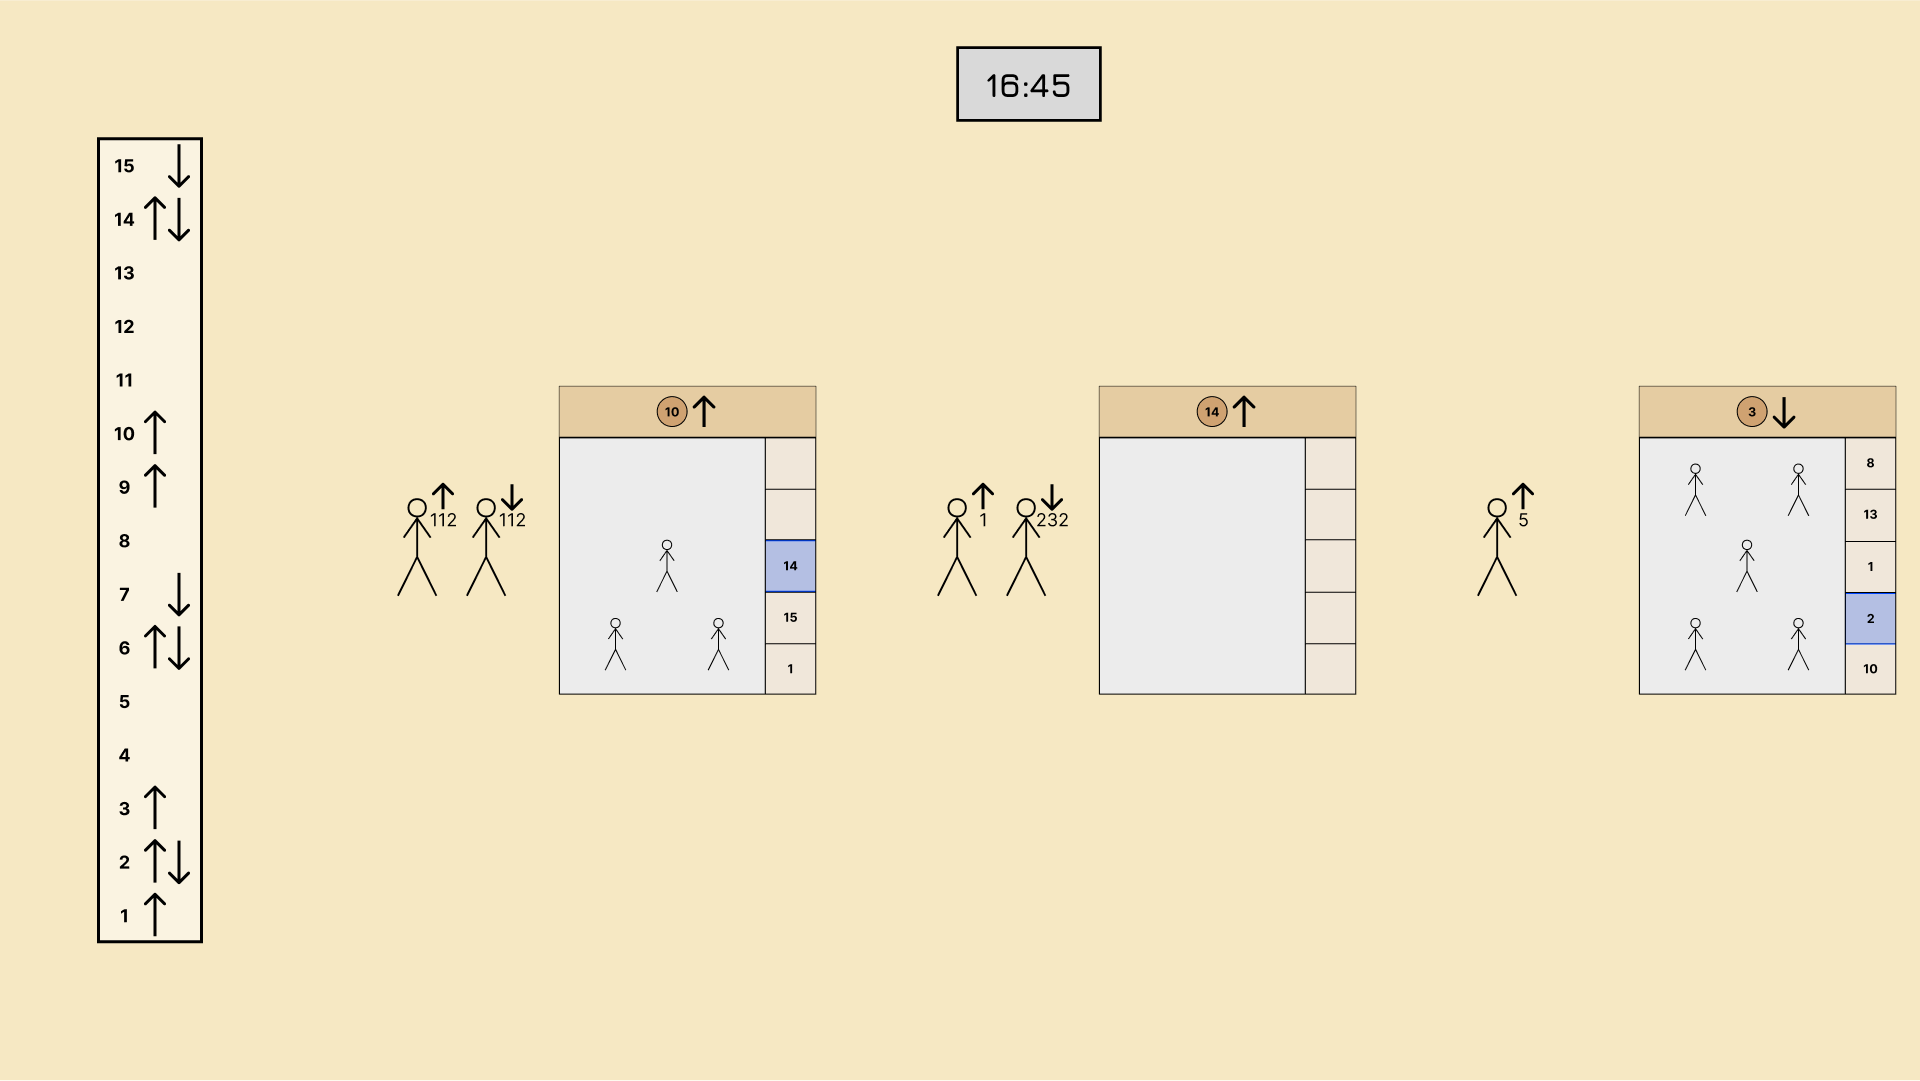
\includegraphics{../images/Fahrstuhl.png}
\caption{UI der späteren Fahrstuhl-Simulation}
\end{figure}

Hierfür wird die Simulation auf einen groben Detailgrad
heruntergebrochen. Die Grenzen der Simulation werden in den
nachfolgenden Kapiteln genauer beleuchtet.

\hypertarget{eigenschaften}{%
\chapter{Eigenschaften}\label{eigenschaften}}

\hypertarget{innere-struktur-des-fahrstuhls}{%
\section{Innere Struktur des
Fahrstuhls}\label{innere-struktur-des-fahrstuhls}}

Der Fahrstuhl ist in 3 Elementen aufgeteilt.

\begin{itemize}
\tightlist
\item
  Stockwerksposition und Fahrtrichtung
\item
  Personenanzahl für nach oben und unten des aktuellen Stockwerks
\item
  Innenraum
\end{itemize}

Der Innenraum zeigt, wie viele Personen sich in ihm befinden und wo
welche Knöpfe in welcher Reihenfolge gedrückt wurden. Des Weiteren wird
sein Fahrziel hervorgehoben angezeigt.

Es gibt drei Zustände je Fahrstuhl:

\begin{itemize}
\tightlist
\item
  Warten
\item
  Hoch
\item
  Runter
\end{itemize}

Warten fasst zwei Zustände zusammen. Das Warten, bis ein Rufknopf
gedrückt wurde und bis der Ein- und Aussteigevorgang abgeschlossen ist.

\hypertarget{uxe4uuxdfere-parameter.}{%
\section{Äußere Parameter.}\label{uxe4uuxdfere-parameter.}}

Die äußeren Parameter, die sich auf das Modell auswirken, sind die zu
befördernden Personen. Die Fahrstühle kennen lediglich die Anzahl der
Personen in ihrem Inneren und in welchem Stockwerk eine unbekannte
Anzahl an Personen nach oben und / oder nach unten möchten. Dabei gilt
ein exponentielles Wachstum.

\hypertarget{ein--und-ausgabeparameter}{%
\section{Ein- und Ausgabeparameter}\label{ein--und-ausgabeparameter}}

Um das Modell möglichst flexibel zu gestalten, wird eine Bandbreite von
Ein- und Ausgabeparametern unterstützt. Diese können wiederum in
Fahrstuhl, Personen und Haus unterteilt werden.

\hypertarget{eingabeparametern}{%
\subsection{Eingabeparametern:}\label{eingabeparametern}}

Zu den Eingabeparametern der Fahrstühle gehören:

\begin{itemize}
\tightlist
\item
  Kapazität der Fahrstühle
\item
  Geschwindigkeit der Etagenwechsel und Dauer des Ein- und
  Aussteigevorgangs (in Takten)
\end{itemize}

Zu den Eingabeparametern des Hauses gehören:

\begin{itemize}
\tightlist
\item
  Anzahl an Etagen
\item
  Liste von Etagen und Zeiten von Spitzenaufkommen (Bspw. Mittagspause).
\end{itemize}

Personen steuern im Gegensatz nur das maximale Tagesaufkommen zu den
Eingaben bei.

\hypertarget{ausgabeparametern}{%
\subsection{Ausgabeparametern:}\label{ausgabeparametern}}

Die Ausgabeparameter beschränken sich außerhalb des Logs lediglich auf
die Aussagen, ob alle Personen bis zum Ende des Tages das Gebäude
verlassen haben und welche durchschnittliche Wartezeit vorliegt.

\hypertarget{verhalten}{%
\chapter{Verhalten}\label{verhalten}}

\hypertarget{vorbedingungen}{%
\section{Vorbedingungen}\label{vorbedingungen}}

Als Vorbedingung der Simulation gelten die Eingangsparameter, die den
Fahrstühlen ihre Eigenschaften beschreiben. Mit den Eigenschaften
repräsentieren die Fahrstühle die Funktionen der Transportation der
Personen auf verschiedenen Stockwerken. Dabei agieren sie nicht aktiv
mit den Personen.

\hypertarget{interne-prozesse}{%
\section{Interne Prozesse}\label{interne-prozesse}}

Die Fahrstühle folgen während der Simulation folgendem Prozessablauf.

\begin{figure}
\centering
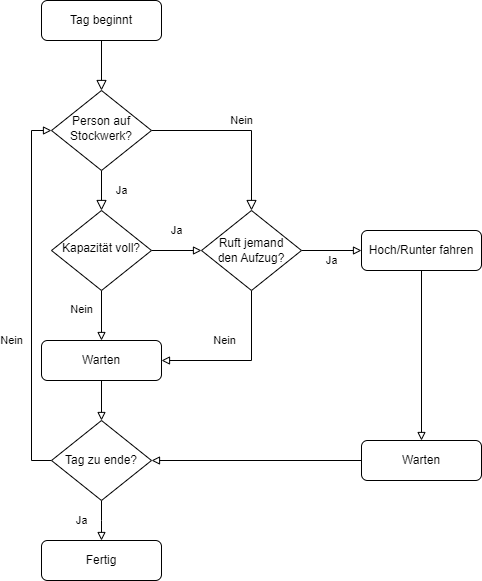
\includegraphics{../images/Simulationstechnik.png}
\caption{Prozessablauf eines Fahrstuhls}
\end{figure}

Zum Beginn wartet ein Fahrstuhl. Hier können zwei Events eintreten. Eine
Person möchte auf dem aktuellen Stockwerk Einsteigen oder der Fahrstuhl
wird von einem anderen Stockwerk aus gerufen. Im zweiten Fall fährt der
Fahrstuhl zum neuen Stockwerk und wartet eine bestimmte Taktzahl
(standardmäßig ein Takt) ab. In dieser Zeit wird der Einstiegsvorgang
simuliert, der auch im ersten Fall vorliegt. Dabei erhöht sich die
Belegung um eins und das gewünschte Stockwerk wird in die Aufgabenliste
eingereiht. Nun entscheidet sich zunächst durch den Aufzug-Algorithmus
(oder auch SCAN) entschieden, welches Stockwerk angefahren werden soll.
Dabei gilt die Zielstockwerke der Insassen und der Personen, die auf die
Stockwerke verteilt den Aufzug rufen. Jedoch kennt der Fahrstuhl nur die
Richtung, in die die Personen außerhalb fahren möchten und nicht deren
Zielstockwerk.

\begin{figure}
\centering
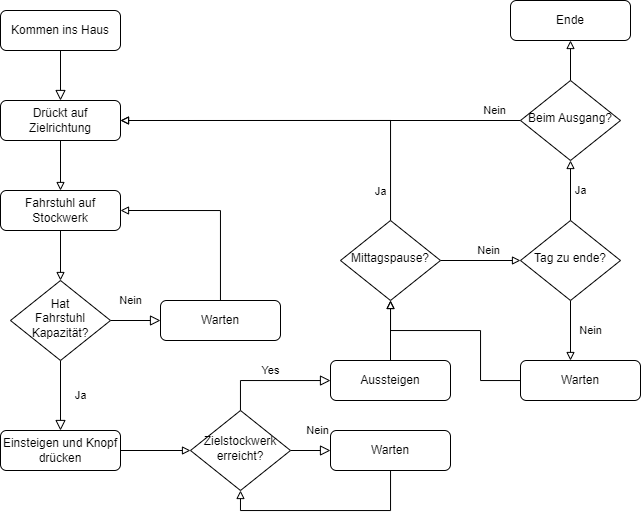
\includegraphics{../images/Simulation_Person.png}
\caption{Prozessablauf einer Person}
\end{figure}

\hypertarget{fehlermuxf6glichkeit}{%
\section{Fehlermöglichkeit}\label{fehlermuxf6glichkeit}}

Die Situation, dass sich am Ende des Tages noch weitere Personen im Haus
befinden, kann als Fehler der Simulation auftauchen. Dies geschieht,
wenn die Fahrstühle zu wenige Personen bedienen konnten. Jedoch lässt
sich dies auch auf ein zu hohes Personenaufkommen zurückzuführen. Diese
Situation tritt vor allem dann auf, wenn selbst das optimale Verhalten
der Fahrstühle nicht ausreicht, um sämtliche Personen zu transportieren.

Daher wird sich für die spätere Optimierung mittels Reinforcement
Learning auf den Personenandrang zurückgegriffen, die bereits der
Aufzug-Algorithmus bewältigen konnte.

\hypertarget{nachbedingung}{%
\section{Nachbedingung}\label{nachbedingung}}

Nach dem Abschluss der Simulation muss als Nachbedingung ein leeres
Gebäude folgen. Keine Person sollte sich noch darin aufhalten.

\hypertarget{verifikation-und-validierung}{%
\chapter{Verifikation und
Validierung}\label{verifikation-und-validierung}}

Um die Simulation abschließend bewerten zur können, benötigt es
Dokumente und Metriken zur Verifikation und Validierung des Programmes.

\hypertarget{verifikation}{%
\section{Verifikation}\label{verifikation}}

Auf die Frage, ob die Simulation richtig implementiert wurde, dient
dieses Conceptual Model als Anforderungen an die Simulation.

\hypertarget{validierung}{%
\section{Validierung}\label{validierung}}

Als Methoden der Validierung werden Behavior Validation und Replicative
Validation angewandt.

Als Behavior Validation wird auf veränderte Parameter ein plausibles
Verhalten erwartet. Im Falle der Fahrstühle wird bei einem erhöhten
Personenaufkommen auch eine höhere durchschnittliche Wartezeit erwartet
und vice versa.

Bei der Replicative Validation werden mittels Experimente die Ergebnisse
verglichen. So soll bei gleichen Parametern trotz Zufallselementen, wie
die Zielstockwerke der Personen, das gleiche oder ein ähnliches Ergebnis
erzielt werden.


% %------------------ Literaturverzeichnis & Index -------------------------------
% \backmatter
% \bibliography{literatur}								% Literaturverzeichnis (literatur.bib)
% \printindex												% Index (optional)


% %------------------ Anhänge ----------------------------------------------------
% \begin{appendix}
% 	\include{chapters/Glossar}							% Glossar (optional)
% 	\include{chapters/Selbststaendigkeitserklaerung}	% Selbstständigkeitserklärung
% \end{appendix}


\end{document}
